% !TEX TS-program = pdflatex
% !TEX encoding = UTF-8 Unicode


\documentclass[11pt]{article} 
\usepackage[utf8]{inputenc} 

%%% PAGE DIMENSIONS
\usepackage{geometry} 
\geometry{letterpaper} 
\geometry{margin=1in} % for example, change the margins to 2 inches all round

\usepackage{graphicx} % support the \includegraphics command and options
\usepackage[parfill]{parskip} % Activate to begin paragraphs with an empty line rather than an indent

%%% HEADERS & FOOTERS
\usepackage{fancyhdr} % This should be set AFTER setting up the page geometry
\pagestyle{fancy} % options: empty , plain , fancy
\renewcommand{\headrulewidth}{0pt} % customise the layout...
\lhead{}\chead{}\rhead{}
\lfoot{}\cfoot{\thepage}\rfoot{}

%%% SECTION TITLE APPEARANCE
\usepackage{sectsty}
\allsectionsfont{\sffamily\mdseries\upshape} % (See the fntguide.pdf for font help)
% (This matches ConTeXt defaults)

%%% END Article customizations



\title{Title TBD}
\author{Author List TBD}
%\date{} % Activate to display a given date or no date (if empty),
         % otherwise the current date is printed 

\bibliographystyle{plain}

\begin{document}
\maketitle

\section{Introduction}
Observations of slow-slip and low-frequency earthquakes in nature suggest that
fault failure encompasses a spectrum of slip modes \cite{Peng:2010, Obara:2002, Ide 2007, Beroza:2011}. While the explanations for
non-traditional earthquakes remain a topic of debate \cite{Kaproth:2013},
an ever increasing pool of data shows them to be found across the globe in a
variety of tectonic settings (REFS). There is currently no way to know if the
large amounts of elastically stored energy in a fault zone will always be
released in slow-slip events or if fault behavior can transition to produce
large earthquakes. It is difficult to study fault zone behavior and evolution
given that large faults may have a recurrence interval of hundreds of years and
that fault slip occurs deep enough in the Earth that we must rely on
instrumentation located kilometers away. Laboratory stick-slip is often used to
model and study repeating earthquake behavior (Brace and Byerlee, 1969; Johnson
et al., 2013). Frictional stability of a system bifurcates at a critical
stiffness , $k_c$ \cite{Gu:1984}. For systems in which
$k>k_c$, linearly stable response, while systems with $k<k_c$ are dynamically
unstable \cite{Scholz:2002}. Behavior at and near $k_c$ is not well understood, but
transitional behaviors such as sinusoidal stress variations and slow-slip have
been observed \cite{Kaproth:2013, Baumberger:1994, Leeman:2015}
Our results show the critical stiffness to be the controlling factor
for slip mode, itself influenced by environmental factors such as pore pressure
and second order frictional properties of the gouge.  

\section{Body}
Biaxial double-direct shearing experiments were performed with humidified
Min-U-Sil\textsuperscript{\textregistered} simulated fault gouge. Force and displacement are recorded on both
axes, as well as a measurement of the shearing block position
(Fig.\ref{Fig:Biax Schematic}). System compliance can be modified by changing
the normal stress or the material of which the shearing block is made (steel
or cast acrylic).  

% Figure %
\begin{figure}
	\centering
	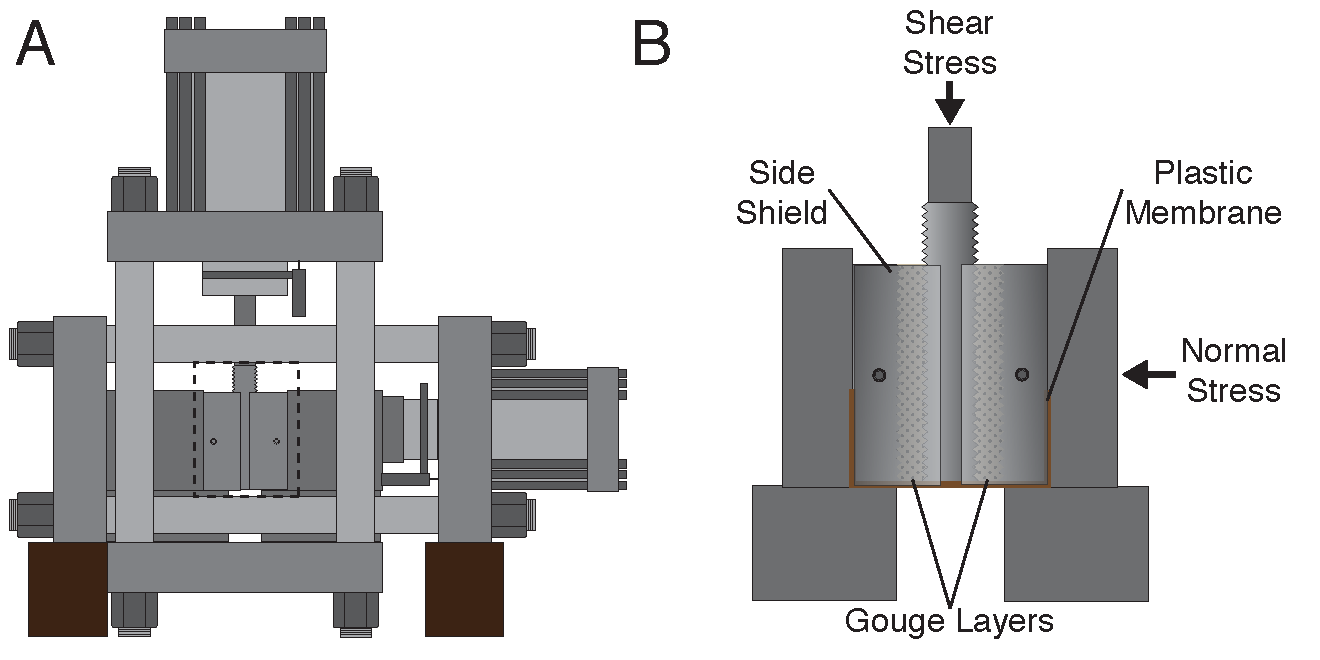
\includegraphics[scale=0.5]{../Figures/Fig_Biax_Schematic/biax_schematic.pdf}
   	\caption{The biaxial deformation apparatus (A) and sample configuration (B). Two large
hydraulic pistons are servo-controlled in either force or displacement control
modes. Double direct shear samples are supported by steel blocks. Samples use
metal side shields and a plastic membrane to reduce gouge extrusion.  Local
displacement transducers (DCDTs) can be referenced to the center block to
negate apparatus stiffness corrections and measure deformation of the
center block.}
  	\label{Fig:Biax Schematic}
\end{figure}
% End Figure %

Experiments performed under stiff system conditions exhibited linearly-stable
behavior in response to order of magnitude velocity perturbations.
Linearly-stable response is characterized by direct matching of the loading and
system velocities and a transitory frictional response. Experiments of identical
conditions, but in a more compliant system exhibited emergent unstable behavior,
beginning with frictional oscillations, and transitioning to dynamic frictional
failure. Oscillations and dynamic failure are characterized by relatively rapid
accelerations and decelerations of the system above/below the load point
velocity when the material yields under excessive shear force. Experiments with
further increased compliance exhibited very rapid dynamic failure that was
audible and classified as fast stick-slip.

System stiffness measured in cycles of unloading and reloading the shear stress
provide an estimate of aggregate stiffness for all experiments regardless of
failure behavior. Stiffnesses recovered from the loading portion of individual
stick-slip events show very low stiffnesses during early frictional oscillations
and emerging slow-slip due to the non-static nature of the system. These values
of “working stiffness” do not represent the overall stiffness of the system, but
a stiffness influenced by continued slip and creep. As dynamic failure reaches a
steady state, we see agreement between the two methods of stiffness measurement.

For experiments exhibiting stable sliding behavior, velocity steps were imposed
to obtain the rate-and-state frictional parameters of the material and system.
The $a$ parameter provides a measure of the direct effect in response to a
velocity step, and $b$ provides the magnitude of friction evolution there-after.
The difference of $a$ and $b$, then yields a quantitative measure of how
strongly velocity strengthening or velocity weakening a material is. The
critical slip distance, Dc, is often considered to be the slip required to renew
the contact population in a granular material. In our experiments, a remains
relatively constant with displacement, but $b$ evolves asymptotically upwards
with increasing shear displacement. During this transitional period, the
critical slip distance evolves downwards.

The transition from velocity strengthening to velocity weakening and
corresponding decrease in $k_c$ increase the value of the predicted critical
stiffness. When the critical stiffness intersects the measured system stiffness,
we begin to see frictional oscillations and dynamic failure. The larger the
departure from $k=kc$, the more dramatic the behavior. Very stiff systems show
no tendency to produced damped oscillations after a velocity step. Very
compliant systems exhibit fast dynamic failure. (Fig. \ref{Figure:Runplot})

% Figure %
\begin{figure}
	\centering
		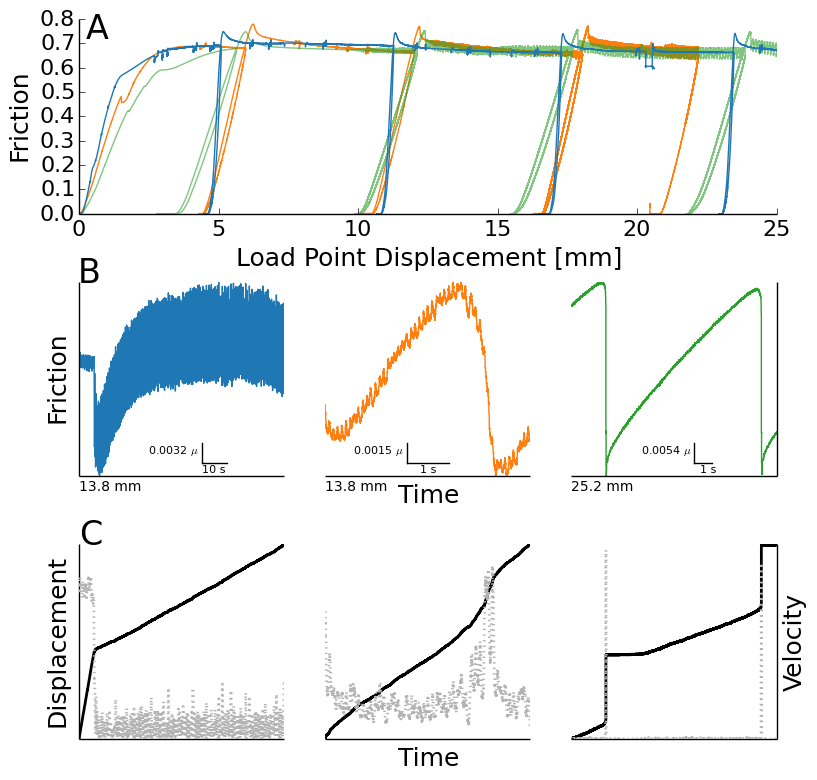
\includegraphics[scale=0.7]{../Figures/Fig_Runplot/runplot.png}
   	\caption{A) Run-plots of experiments p4309 (blue), p4311 (orange), and p4316 (green).
Different working stiffnesses can be observed as the slope of unload/reload
segments. B) All steel blocks produced stable responses to velocity steps.
C) Destiffening the system with an acrylic center block produced non-audible
slow-slip events. D) Further destiffening with an acrylic center block and
increased normal stress produced audible fast stick-slip events.   }
  	\label{Figure:Runplot}
\end{figure}
% End Figure %

An examination of the requirements for unstable behavior yields two suggested
conditions: 1) that the material be velocity neutral to velocity weakening, and
2) that the system stiffness be at or below the critical stiffness. Velocity
weakening is a necessary, but insufficient condition for unstable behavior. If a
material is velocity strengthening, any acceleration leading to slip is
immediately arrested by increased shearing resistance. The stiffness of the
system governs the rate at which energy stored as strain can be released. If the
energy release occurs in such a way that the drop in shear resistance with
displacement occurs faster than the drop in applied shearing force with
displacement, the system can support unstable failure.

% Figure %
\begin{figure}
	\centering
		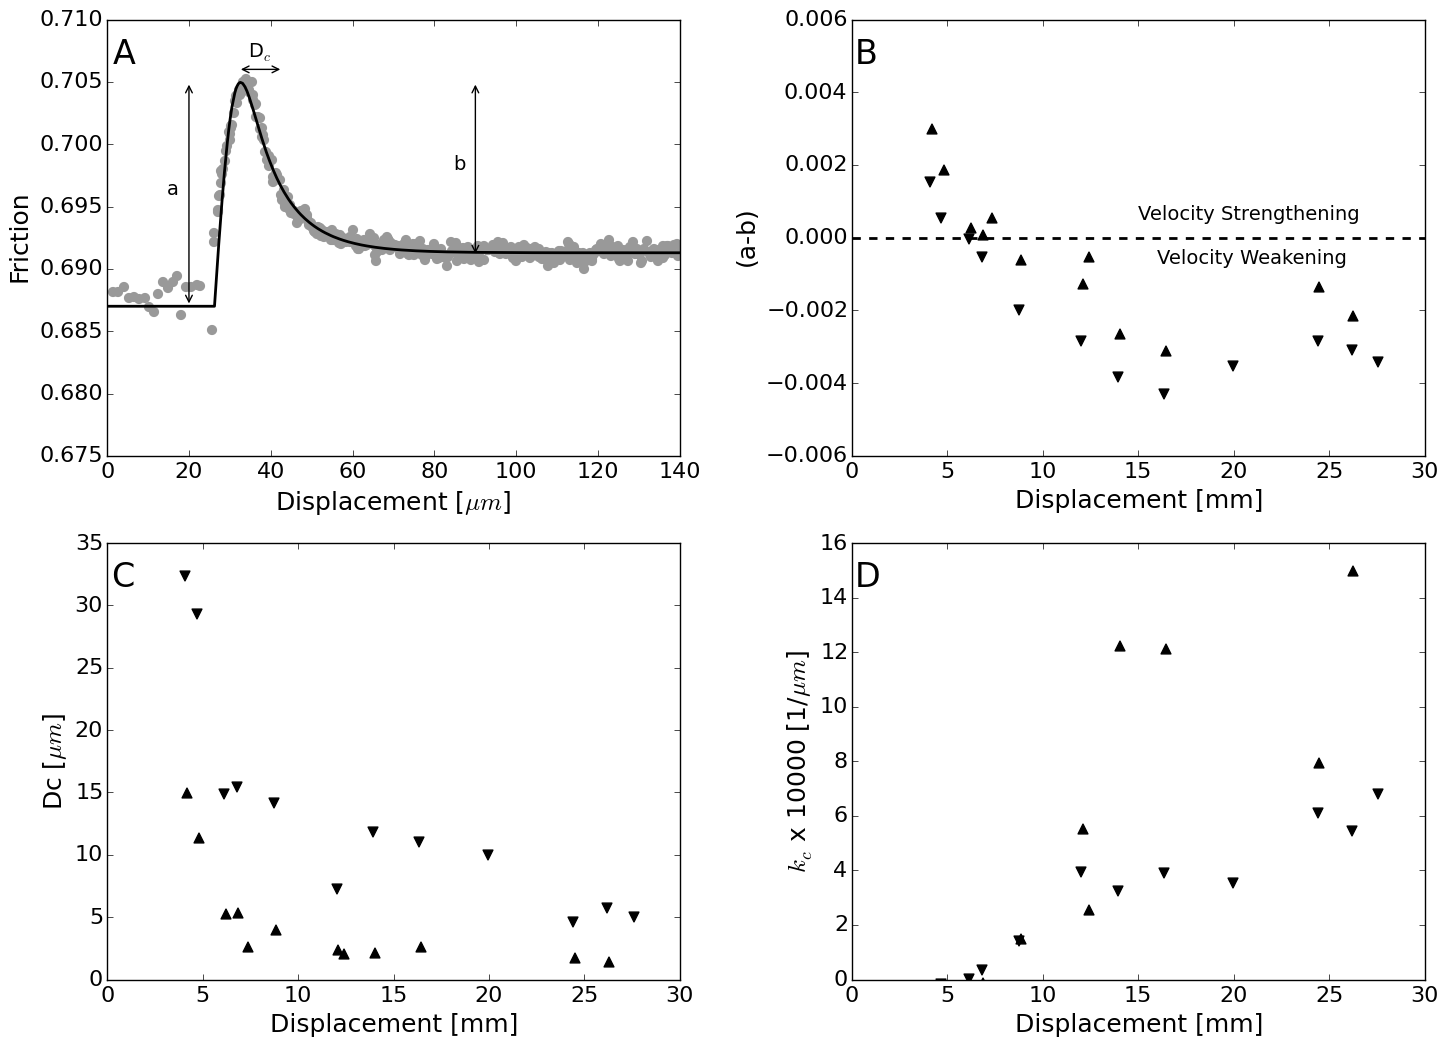
\includegraphics[scale=0.45]{../Figures/Fig_RSF_Parameters/RSF_Parameters.png}
   	\caption{Rate-and-state friction parameters obtained from velocity step inversions. All
inversions were accomplished with a fixed stiffness of 5.5e-3/um. A) rate-and-state
parameter a remains relatively constant with displacement and shows a systematic
behavior with higher values of a always being observed during velocity
up-steps. The b parameter shows a similar behavior, but also increases with
displacement, reaching a steady-state value around 10 mm displacement.
B) The sample transitions from velocity strengthening to velocity weakening
 behavior at around 10 mm and remains velocity weakening for the remainder of
 the experiment. C) Critical slip distance estimates show considerable scatter,
 but do reduce to a steady-state value of 5-10 um.  }
  	\label{Figure:RSF Props}
\end{figure}
% End Figure %

\section{Discussion}
Increases in measured aggregate system stiffness could be due to layer
compaction due to grain rearrangement, layer thinning with increased shear
strain, possible grain comminution and increased packing, localization of shear,
and reduction of compliant material above sample due to geometric effects with
shear. Of these, layer compaction, thinning, and shear localization are believed
to be the largest.  

Our observations of transitional behavior beginning when $k \sim k_c$ suggests
that $k_c$ is a valid proxy for the stability of a system, marking a transitory
zone between stable sliding and stick-slip that encompasses slow-slip and
oscillatory behavior. We also observe that the critical stiffness of a system
evolves with shear strain, suggesting that tectonic faults may change behavior
as they accumulate slip and become mature fault zones. Laboratory results can
also be connected to observations in nature through the critical patch size.
Critical patch size grows with increasing $k_c$ and/or increasing normal stress.
Extending this to large patch sizes hypothesized for slow-slip events suggests
lowered normal stress, possibly due to high pore-pressures and/or low critical
stiffness values.

\section{Methods}
All experiments were performed on a servo-controlled biaxial shearing apparatus.
Displacements on the normal and shearing axes were measured by Direct Current
Displacement Transducers (DCDTs) referenced at the end-platens and ram nose. The
displacement of the shearing block was measured with a DCDT referenced at the
end-platen and the top of the shearing block. Loads applied to the sample were
measured with strain gauge load cells. All transducers are semi-annually
calibrated with a traceable transfer standard.

Samples were prepared in the double-direct-shear geometry using steel or
titanium side blocks and steel or acrylic shearing blocks. All blocks were
grooved 0.8 mm deep at 1 mm spacing to reduce boundary effects. The sample area
was 10 x 10 cm and filled with Min-U-Sil to a thickness of 3 mm. Granular layers
were left in a sealed container overnight with a solution of anhydrous sodium
carbonate to humidify the samples.

After samples were loaded into the load frame, a constant normal stress was
applied and maintained by the servo system in a force feedback control mode.
Samples were allowed to compact and accomodate grain rearrangement before
shearing began. Shearing is conducted at a fixed rate of 10 $\mu m/s$ in
displacement feedback control mode.

Stiffness of the system was altered by changing the applied normal stress and by
changing the material of the shearing block. Increasing normal stress decreases
the effective stiffness of the system, as does switching the steel forcing block
for a cast acrylic block.

Layers were built of Min-U-Sil\textsuperscript{\textregistered} 40 fine ground silica from the U.S. Silica\textsuperscript{\textregistered}
company Berkeley Springs, West Virginia plant. The median diameter of grain is
10.5 $\mu m$. The product is 99.5 \% SiO$_s$, with traces of metal oxides making
up the remainder.

System stiffnesses from unload/reload shear stress cycles were calculated by a
least-squares linear fit in friction vs. displacement for the interval $\mu =
0.3-0.4$. Stiffnesses from the loading portion of slow-slip and stick-slip
events were obtained with a derivative based algorithm described by Leeman et
al. (In Review). Rate-and-state models were fit with both the Dieterich and
Ruina laws, with comparable results. Inversions were done with an iterative
singular value decomposition technique.  

\section{References}
\bibliography{references}

\section{Acknowledgements}
The authors with to thank Steve Swavely for his support in the laboratory. This
material is based upon work supported by the National Science Foundation under
Grant No. DGE1255832.  Any opinions, findings, and conclusions or
recommendations expressed in this material are those of the author(s) and do not
necessarily reflect the views of the National Science Foundation. The work was
also supported by funds from the GDL Foundation and Shell Oil.

\section{Author Contributions}
All authors contributed to data interpretation, analysis schema, and writing.
J. Leeman conducted experiments and data analysis.

\section{Competing Financial Interests}
The authors declare no competing financial interests. Supplementary information
accompanies this paper on www.nature.com/naturegeoscience. All data is avaliable
for download, as well as Python scripts/notebooks to replicate data analysis on
GitHub (www.github.com/jrleeman). Reprints and permissions information is
available online at http://npg.nature.com/reprintsandpermissions. Correspondence
and requests for materials should be addressed to J. Leeman.  

\end{document}




